In this section, we describe the measurement model for a single-pixel
time-of-flight lidar sensor under diffuse, pulsed laser illumination. 
\subsection{Measurement Model}
Consider a laser which emits a pulse at time $t = 0$ with time-varying intensity
$g(t)$ uniformly illuminating some 3D scene. We parameterize the geometry of the
scene as a height map $z(x, y)$.
Neglecting albedo and falloff effects, an ideal detector counting photon events
from a location $(x,y)$ in the time interval $(n\Delta t, (n+1) \Delta t)$ would record

\begin{equation}
  \lambda_{x,y}[n] = \int_{n\Delta t}^{(n+1) \Delta t} (f * g)\paren*{t - 2z(x,y)/c} dt \label{single_loc_spad} 
\end{equation}  

where $c$ is the speed of light, and $f$ is a function that models the temporal uncertainty in the
detector. Single-photon avalanche diodes (SPADs) are highly sensitive
photodetectors which are able to record single photon events with high temporal
precision \cite{Stuff}. Since the event corresponding to the detection of a
photon can be described with a Bernoulli random variable,
the total number of accumulated photons in this time interval follows a Poisson
distribution according to

\begin{equation}
  h[n] \sim \mathcal{P}\paren*{\sum_{x,y}\alpha_{x,y}\eta \lambda_{x,y}[n] + b} \label{global_hints}
\end{equation}

where $\alpha_{x,y} = r_{x,y}/z(x,y)^2$ captures the attenuation of the
photon counts due to the reflectance $r(x,y)$ of the scene and due to the
inverse square falloff $1/z(x,y)^2$.
In addition, $\eta$ is the detection probability of a photon
triggering a SPAD event, and $b = \eta a + d$ is the average number of background detections resulting
from ambient photons $a$
and erroneous ``dark count'' events $d$ resulting from noise within the SPAD.
% \newpage
% \begin{table*}[htbp]
%   \begin{center}
  %   \begin{tabularx}{\linewidth}{*{2}{X}}
  %     \includegraphics[width=\textwidth/2-5pt]{sections/figures/spad_example/rgb.png} &
  %     \includegraphics[width=\textwidth/2-5pt]{sections/figures/spad_example/rawdepth.png} \\
  %     \includegraphics[width=\textwidth/2-5pt]{sections/figures/spad_example/depth_hist.png} &
  %     \includegraphics[width=\textwidth/2-5pt]{sections/figures/spad_example/spad_hist.png} \\
  %   \end{tabularx}
  % \end{center}
  % \caption{Sample Image. Top Left is the RGB image. Top Right is ground truth
  %   depth. Bottom Left is Raw ground truth depth histogram. Bottom Right is
  %   simulated SPAD measurements. Notice how closer depths are magnified and far
  %   depths are attenuated.}
% \end{table*}

\subsection{Monocular depth estimation with global depth hints}
Given a single RGB image $I(x,y)$ and a vector of photon arrivals $h[n]$
described by equation \ref{global_hints}, we seek to
reconstruct the ground truth depth map $z(x,y)$.
Our method has two parts. First, we \textbf{initialize} our estimate of the depth map from the single RGB
image via a monocular depth estimator described below. Second, we \textbf{refine} this depth map using
the captured measurements $h[n]$ via exact histogram matching. 

\paragraph{Initialization}
The first step in our method is to produce an initial estimate of ground truth
depth. Convolutional Neural Networks have been shown to produce accurate, if poorly-scaled, estimates of depth
from only a single image. We therefore choose to initialize our depth map
estimate $\hat z^{(0)}(x,y)$ using
a CNN. However, any depth estimator reliant on only a single
view may be used for this step. Furthermore, in the larger context of our
algorithm, it is more important that the network predict the correct ordinal
relationships between pixels - that is, to predict the correct relative ordering
of pixels $a$ and $b$, rather than to get all pixels exactly correct.

\paragraph{Exact Histogram Matching}
\begin{figure}
  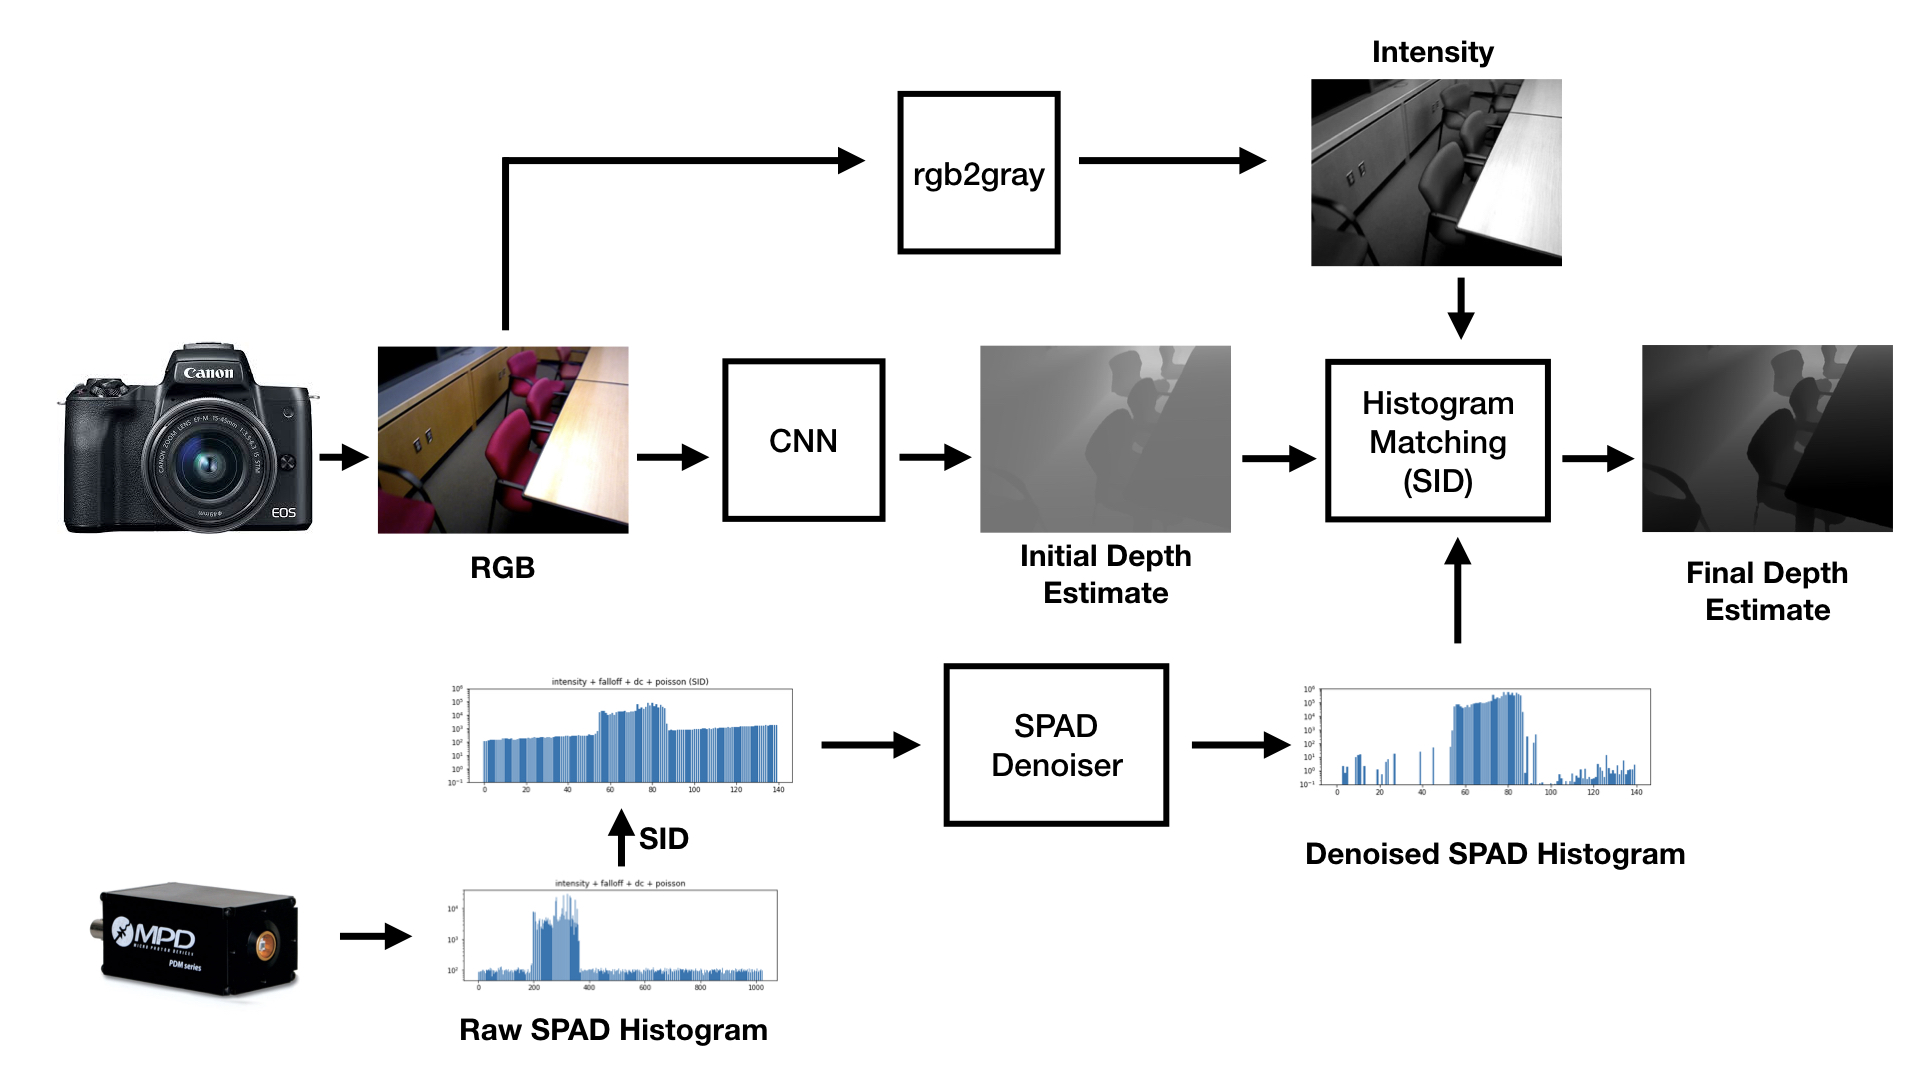
\includegraphics[width=\textwidth/2]{sections/figures/full_pipeline/full_pipeline.jpeg}
  \caption{\textbf{Overview of the full pipeline} We use a CNN to get an initial
  per-pixel depth estimate. Then we perform exact histogram matching using
  intensity-weighted pixel values on the corrected SPAD data.}
\end{figure}
An image's \textit{histogram} is a pair of vectors $(h, b)$ where $h_i$ is the number of
pixels of the image whose value lies in the range $[b_i, b_i+1)$.
Then, given a source image $S$ with histogram $(h_s, b)$ and a target histogram
$(h_t, b)$, histogram matching generates a new image $M$ such that $h_m \approx
h_t$ and the pixel values in $M$ are in the same relative order as in $S$.
The full details of the exact histogram matching algorithm can be found in
\cite{Morovic2002}.

However, for our purposes, we need to modify our algorithm to accommodate
differing per-pixel weights. We can account for squared depth falloff

\paragraph{SPAD Denoising}
\begin{itemize}
  \item Talk about histogram matching in the ideal case, jump straight to intensity 
  \item Talk about histogram matching in our case, and how it approaches the
    ideal case. Discuss the following corrections 
    \begin{itemize}
      \item Ambient/DC - Use \cite{Xin2019} to justify looking for large edges,
        then the ambient estimate to get rid of the noise floor.
      \item Falloff
    \end{itemize}
  \item Talk about how the histogram matching works with intensity
    considerations applied, briefly.
  \item We don't address jitter or poisson noise.
\end{itemize}
\begin{equation}
  h[n] \sim \mathcal{P}\paren*{\sum_{x,y}\alpha_{x,y}\eta \lambda_{x,y}[n] + b} \label{global_hints}
\end{equation}
Given a SPAD with histogram $h$ according to the above equation, we first
process the SPAD to remove the effects of some of the terms. First, we 
\subsection{Implementation Details}
For the Monocular Depth Estimator, we use pretrained versions of the
the Deep Ordinal Regression Network (DORN) \cite{} and the DenseDepth Network.
The exact histogram matching method is as described in \cite{}.


